\documentclass[11pt,a4paper]{article}
\usepackage[T1]{fontenc}
\usepackage[utf8]{inputenc}
\usepackage[italian]{babel}
\usepackage{lmodern}
\usepackage{microtype}
\usepackage[margin=2.5cm]{geometry}
\usepackage{amsmath,amssymb}
\usepackage{graphicx}
\usepackage{booktabs}
\usepackage{tabularx}
\usepackage{enumitem}
\usepackage{caption}
\usepackage{float}
\usepackage{tikz}
\usetikzlibrary{arrows.meta,positioning,calc}
\usepackage[hidelinks]{hyperref}
\setlist{itemsep=2pt,topsep=4pt}
\captionsetup{font=small,labelfont=bf}
\setlength{\parskip}{4pt}
\setlength{\parindent}{0pt}
\setlength{\emergencystretch}{2em}
\newcommand{\dire}[1]{\par\noindent\textbf{In una frase.} #1\par}
\newcommand{\attenzione}[1]{\par\noindent\textbf{Limiti.} #1\par}

\title{\textbf{Q-Spy}: kernel quantistici proiettati, consapevoli della concentrazione,\\
per la classificazione few-shot e la novelty detection dei glitch LIGO\\[4pt]\large Report tecnico (L-06)}
\author{Team Q-Spy}
\date{25 novembre 2026}

\begin{document}
\maketitle

\begin{abstract}
\noindent Studiamo se un kernel quantistico proiettato, calcolato su un processore IBM reale, aiuta a classificare
famiglie di glitch di LIGO con pochi esempi e a riconoscere una famiglia mai vista (Fast Scattering). Le 7 feature
Omicron di ogni glitch sono codificate in un circuito di 8 qubit con entanglement; i vettori di Bloch misurati
definiscono il kernel, usato da SVM e One-Class SVM classiche. In simulazione esatta il kernel proiettato si concentra
meno del fidelity kernel e la bandwidth della codifica è la variabile dominante (KTA 0,534 contro 0,357). Su
\texttt{ibm\_kingston}, con mitigazione, l’errore dei vettori di Bloch è pari al rumore di campionamento (0,030) e
l’allineamento con le classi resta entro 0,006 da quello esatto (H4 supportata). Nel few-shot il kernel proiettato è
alla pari con un RBF classico; nella novelty detection l’RBF classico è migliore di 0,026 di AUROC (H3 non supportata).
Configurazione, ipotesi e sottoinsiemi hardware sono stati fissati prima delle misure (tag \texttt{hw-freeze}); ogni
numero è riconducibile a uno script e a un run (appendice~\ref{app:numeri}).
\end{abstract}

\section{Introduzione}
I glitch sono transitori di rumore non gaussiano nei rivelatori LIGO che degradano la sensibilità e possono imitare
segnali. Gravity Spy li classifica con reti convoluzionali e citizen science (Zevin et al.\ 2017), ma le famiglie nuove,
come Fast Scattering in O3, emergono dal lavoro umano (Soni et al.\ 2021; Glanzer et al.\ 2023). Due problemi restano
aperti: imparare una famiglia con pochi esempi e segnalare una famiglia sconosciuta. Sul lato quantistico, i kernel
quantistici (Havlíček et al.\ 2019; Schuld e Killoran 2019) soffrono di concentrazione esponenziale (Thanasilp et al.\
2024); i kernel proiettati la attenuano (Huang et al.\ 2021), ma confronti accurati con baseline classiche spesso non
mostrano vantaggi (Bowles et al.\ 2024) e i modelli non concentrati possono essere simulabili (Cerezo et al.\ 2023).
Questo report misura entrambi gli aspetti su dati veri e su hardware reale, con un protocollo pre-registrato.

\section{Dati e metodo}
\textbf{Dati.} Catalogo Gravity Spy O1--O3b curato (D-02): confidenza $\geq0{,}9$, duplicati tra rivelatori entro
0,1\,s rimossi; 318.801 glitch in 8 famiglie, Fast Scattering solo in O3 e quasi tutta su L1. Split congelati e
verificati con hash (D-04): P1 few-shot ($k\in\{5,10,20,50\}$), P2 novelty (una famiglia nascosta, Fast Scattering
nel caso principale).

\textbf{Feature e codifica.} Sette feature Omicron (durata, frequenza di picco e centrale, banda, ampiezza, SNR,
fattore Q): $\log_{10}$, RobustScaler stimato sul solo training, clipping in $[-1,1]$. Angoli $\theta=s\pi\tilde x$;
per strato $R_Y(\theta)R_Z(\theta)$ su ogni qubit (feature $q\bmod7$) e catena di CZ a mattoni; 2 strati, 8 qubit,
profondità a 2 qubit 4 su \texttt{ibm\_kingston}.

\textbf{Kernel e modelli.} $k_P(x,x')=\exp(-\tfrac{\gamma}{n}\sum_q\lVert b_q(x)-b_q(x')\rVert^2)$ sui vettori di Bloch;
confronto con RBF sulle feature, Isolation Forest e LOF. Budget di ricerca uguale per i modelli confrontati;
$\gamma=c/\text{mediana}$ delle distanze quadratiche, $c\in\mathrm{logspace}(-2,2,9)$. Novelty: selezione
leave-one-family-out annidata sulle famiglie note, soglia al 5\% di falsi allarmi sui noti.

\textbf{Livelli.} L0 statevector, L1 1112 shot, L2 emulatore con il modello di rumore di \texttt{ibm\_kingston}, HW
\texttt{ibm\_kingston} via Qiskit Runtime EstimatorV2 con TREX, twirling e dynamical decoupling.

\section{L’idea in una pagina}

\textbf{Domanda.} Un kernel quantistico, calcolato su un chip IBM reale, aiuta a riconoscere famiglie di glitch con
pochi esempi e a scoprire una famiglia nuova? E prima ancora: resta informativo (non si concentra) e sopravvive al
rumore dell’hardware?

\textbf{Risposta breve.} Il kernel proiettato si concentra meno del fidelity kernel e, alla bandwidth giusta, porta
informazione sulle classi. Sul chip IBM, con mitigazione, i vettori misurati hanno lo stesso errore del solo
campionamento e conservano la stessa informazione della simulazione. Ma su queste 7 feature tabellari un metodo
classico ben tarato fa uguale (few-shot) o un po’ meglio (novelty). Nessun vantaggio quantistico: un risultato
negativo misurato con regole fissate prima.

\begin{figure}[H]
\centering
\begin{tikzpicture}[
  box/.style={draw, rounded corners=3pt, align=center, minimum height=1.3cm, text width=2.0cm, font=\small},
  q/.style={box, very thick, draw=teal},
  arr/.style={-{Latex}, thick}]
  \node[box] (d) {7 feature\\Omicron};
  \node[box, right=0.38cm of d] (f) {log, scaler\\robusto, clip\\$\tilde x\in[-1,1]$};
  \node[q, right=0.38cm of f] (c) {circuito\\8 qubit\\$\theta=s\pi\tilde x$};
  \node[q, right=0.38cm of c] (m) {misura\\$\langle X\rangle,\langle Y\rangle,\langle Z\rangle$\\24 numeri};
  \node[box, right=0.38cm of m] (k) {kernel\\proiettato\\$k_P$};
  \draw[arr] (d) -- (f); \draw[arr] (f) -- (c); \draw[arr] (c) -- (m); \draw[arr] (m) -- (k);
  \node[box, below=1.0cm of k, text width=3.4cm] (svm) {SVM (few-shot)\\One-Class SVM (novelty)};
  \draw[arr] (k) -- (svm);
  \node[box, left=1.2cm of svm, text width=3.6cm] (store) {store: vettori di Bloch\\con hash e commit};
  \draw[arr, dashed] (m.south) -- ++(0,-0.4) -| (store.north);
  \node[font=\small, teal] at ($(c.north)!0.5!(m.north)+(0,0.4)$) {parte quantistica};
\end{tikzpicture}
\caption{La pipeline. Solo i due blocchi con il bordo spesso girano sul chip (o sul simulatore); tutto il resto è
classico. L’interfaccia tra i due mondi sono i vettori di Bloch salvati nello store.}
\label{fig:pipeline}
\end{figure}

\section{Come si rapportano quantum e machine learning}
È il punto concettuale da saper spiegare meglio, perché è la risposta a “dove sta il quantum ML?”.

\begin{center}
\begin{tabularx}{\textwidth}{@{}>{\raggedright\arraybackslash}X>{\raggedright\arraybackslash}X@{}}
\toprule
\textbf{Quantum (chip o simulatore)} & \textbf{Machine learning (classico)}\\
\midrule
codifica le 7 feature in uno stato di 8 qubit & sceglie lo scaler sul solo training\\
misura 24 numeri per glitch, una sola volta & sceglie $\gamma$, $C$, $\nu$ con validazione annidata\\
nessun parametro allenato sul chip & allena SVM e One-Class SVM sul kernel\\
costo fissato in anticipo (3 circuiti per glitch) & calibra le soglie, misura e confronta\\
\bottomrule
\end{tabularx}
\end{center}

\textbf{La frase chiave:} il chip cambia la \emph{geometria} in cui confrontiamo i glitch; il machine learning decide
come usarla. È un modello \emph{ibrido} del tipo “quantum kernel”: diverso dalle reti neurali quantistiche variazionali,
dove si ottimizzano i parametri del circuito sul chip con i gradienti. Noi non ottimizziamo niente sul chip, quindi:
niente barren plateau (gradienti che spariscono), niente ciclo di ottimizzazione costoso sulla QPU, e un costo
calcolabile prima di partire. Il prezzo è che il circuito è fisso: tutta la flessibilità sta nei parametri classici
($s$ scelto in simulazione, $\gamma$, $C$, $\nu$ scelti dopo la misura).

\textbf{Come si vede l’effetto del quantum:} mettiamo la \emph{stessa} SVM su due geometrie diverse, quella
quantistica (kernel proiettato sui vettori di Bloch) e quella classica (RBF sulle 7 feature). Se il modello quantistico
fa meglio a parità di tutto il resto, il merito è della geometria quantistica.

\section{Le regole: livelli, pre-registrazione, ipotesi}

\subsection{Quattro livelli di realismo}
\begin{center}
\begin{tabularx}{\textwidth}{@{}l>{\raggedright\arraybackslash}X>{\raggedright\arraybackslash}X@{}}
\toprule
Livello & Cosa è & A cosa serve\\
\midrule
L0 & simulazione esatta (statevector) & la verità di riferimento\\
L1 & simulazione con 1112 shot & quanto pesa il solo campionamento\\
L2 & emulatore con il rumore di \texttt{ibm\_kingston} & prevedere l’hardware (senza mitigazione: pessimista)\\
HW & chip vero, con mitigazione & la misura\\
\bottomrule
\end{tabularx}
\end{center}

\subsection{Pre-registrazione}
Prima di usare il chip abbiamo congelato tutto in \texttt{configs/hardware\_frozen.yaml} (tag git \texttt{hw-freeze}):
8 qubit, 2 strati, $s=0{,}1778$, precisione 0,03, i sottoinsiemi di glitch (D-05), e quattro ipotesi con il loro test
(\texttt{docs/decisions.md}). Serve a non scegliere a posteriori la configurazione che “viene meglio”.

\begin{center}
\begin{tabularx}{\textwidth}{@{}l>{\raggedright\arraybackslash}X>{\raggedright\arraybackslash}p{4.3cm}@{}}
\toprule
& Ipotesi & Stato oggi\\
\midrule
H1 & few-shot: il kernel proiettato non è peggiore dell’RBF classico ($k\leq10$) & anteprima su 5 seed: alla pari; test completo da fare (20 seed, Wilcoxon)\\
H2 & l’entanglement aiuta: con le CZ meglio che senza & non ancora testata\\
H3 & novelty: OC-SVM proiettato ha AUROC più alto dell’OC-SVM RBF su Fast Scattering & \textbf{non supportata} in L0: $-0{,}026$ $[-0{,}044;\,-0{,}008]$\\
H4 & hardware: la KTA sul chip resta entro 0,02 da quella esatta & \textbf{supportata}: $-0{,}006$ $[-0{,}010;\,-0{,}001]$\\
\bottomrule
\end{tabularx}
\end{center}

\section{I risultati, figura per figura}

Per ogni risultato: la domanda, come è stato fatto, come leggere la figura, cosa dire, a cosa stare attenti.

\subsection{Risultato 1 --- concentrazione sui dati veri (E-01)}
\textbf{Domanda.} Con quali qubit, profondità e bandwidth il kernel rappresenta meglio i glitch senza concentrarsi?
\textbf{Come.} 196 glitch veri (28 per famiglia nota), simulazione esatta di una griglia di 468 configurazioni:
$n=4,6,\dots,16$ qubit, $L=1,2,4,8$ strati, 9 valori di $s$ tra 0,03 e 3, per entrambi i kernel (fidelity fino a 14 qubit).

\begin{figure}[H]
\centering
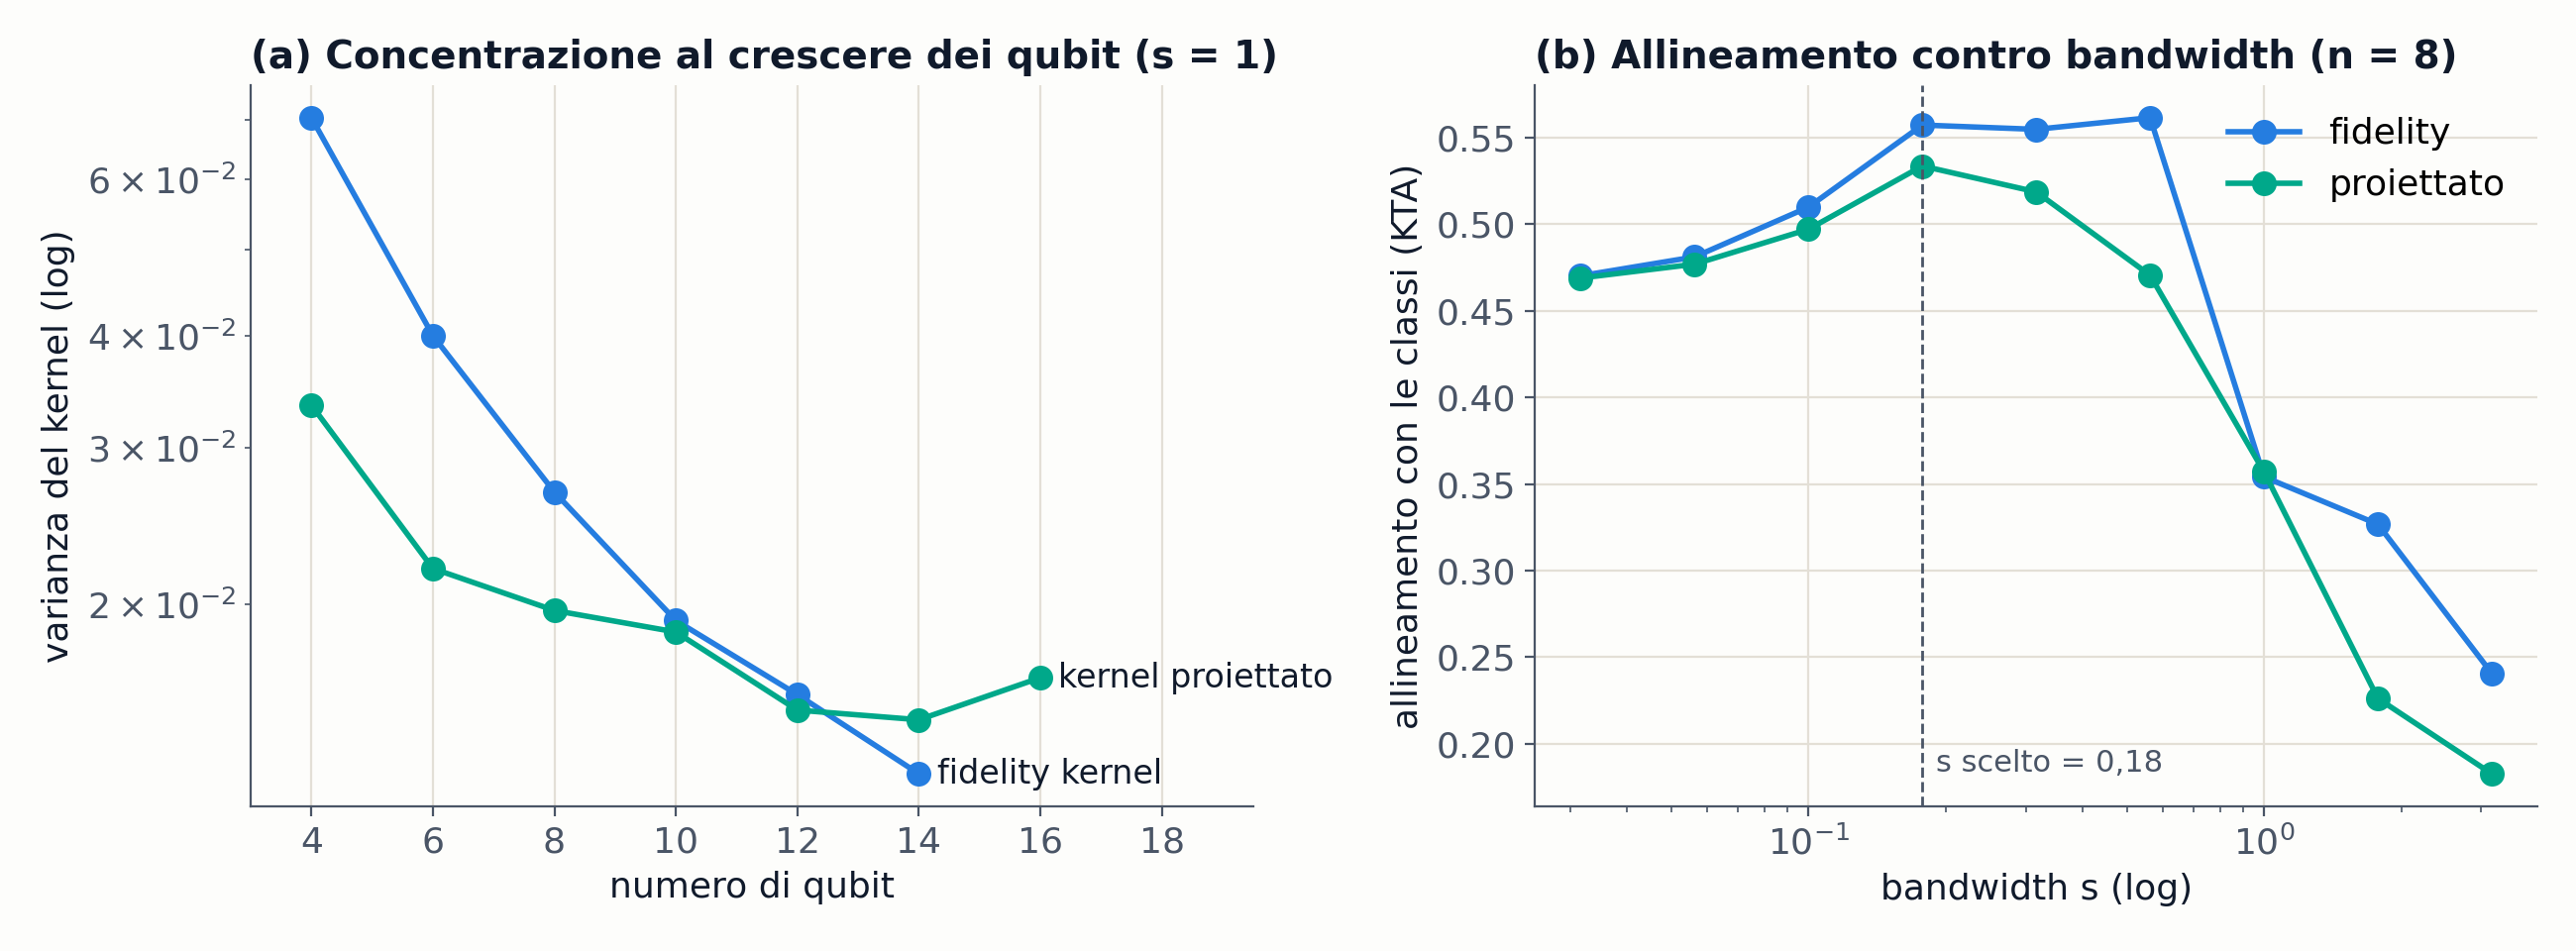
\includegraphics[width=\textwidth]{fig/e01_slide.png}
\caption{E-01. (a) Varianza dei valori del kernel fuori diagonale contro il numero di qubit, a $s=1$, 2 strati.
(b) Allineamento con le famiglie (KTA) contro la bandwidth $s$, a 8 qubit e 2 strati.}
\label{fig:e01}
\end{figure}

\textbf{Come leggere (a).} In ordinata c’è la varianza dei valori del kernel tra coppie diverse, in scala logaritmica.
Se scende verso zero, il kernel dà lo stesso valore a tutte le coppie: è la concentrazione. Il fidelity kernel (blu)
scende di circa 6 volte da 4 a 14 qubit; il proiettato (verde) scende di circa 2 volte fino a 6 qubit e poi si
stabilizza. La concentrazione è più lieve del caso peggiore teorico perché le feature distinte sono solo 7 e oltre 7
qubit si ripetono.

\textbf{Come leggere (b).} È la figura chiave. Con $s$ piccolo gli stati restano tutti vicini a $|0\rangle$ e
l’allineamento è basso; c’è un picco tra $s\approx0{,}18$ e $0{,}56$; sopra $s=1$ crolla per entrambi i kernel.
La linea tratteggiata è il valore scelto. A $s=0{,}1778$ il proiettato vale 0,534 contro 0,357 a $s=1$ (il valore
usato nel pilota): scegliere bene la bandwidth vale il 50\% di allineamento in più.

\dire{“La concentrazione è reale: il fidelity kernel perde varianza molto più in fretta. Ma la variabile che conta di
più non è il numero di qubit, è la bandwidth. L’abbiamo scelta qui, in simulazione, prima di toccare l’hardware.”}

\attenzione{a 8 qubit il fidelity kernel si allinea un po’ meglio del proiettato (0,557 contro 0,534). Lo abbiamo
scartato per il costo sull’hardware, non per la qualità. Da 8 a 12 qubit l’allineamento non cambia; a 14--16 sale
di poco (0,555 e 0,570), ma raddoppia i qubit rumorosi: per questo 8.}

\subsection{Risultato 2 --- rumore previsto prima dell’hardware (Q-06)}
\textbf{Domanda.} Con la configurazione scelta, il rumore cancellerà le differenze tra glitch? Che precisione serve?
\textbf{Come.} I 120 glitch “main” della campagna (15 per famiglia, Fast Scattering compresa, mai visti in training),
nei livelli L0, L1, L2, per quattro combinazioni di bandwidth e precisione.

\begin{figure}[H]
\centering
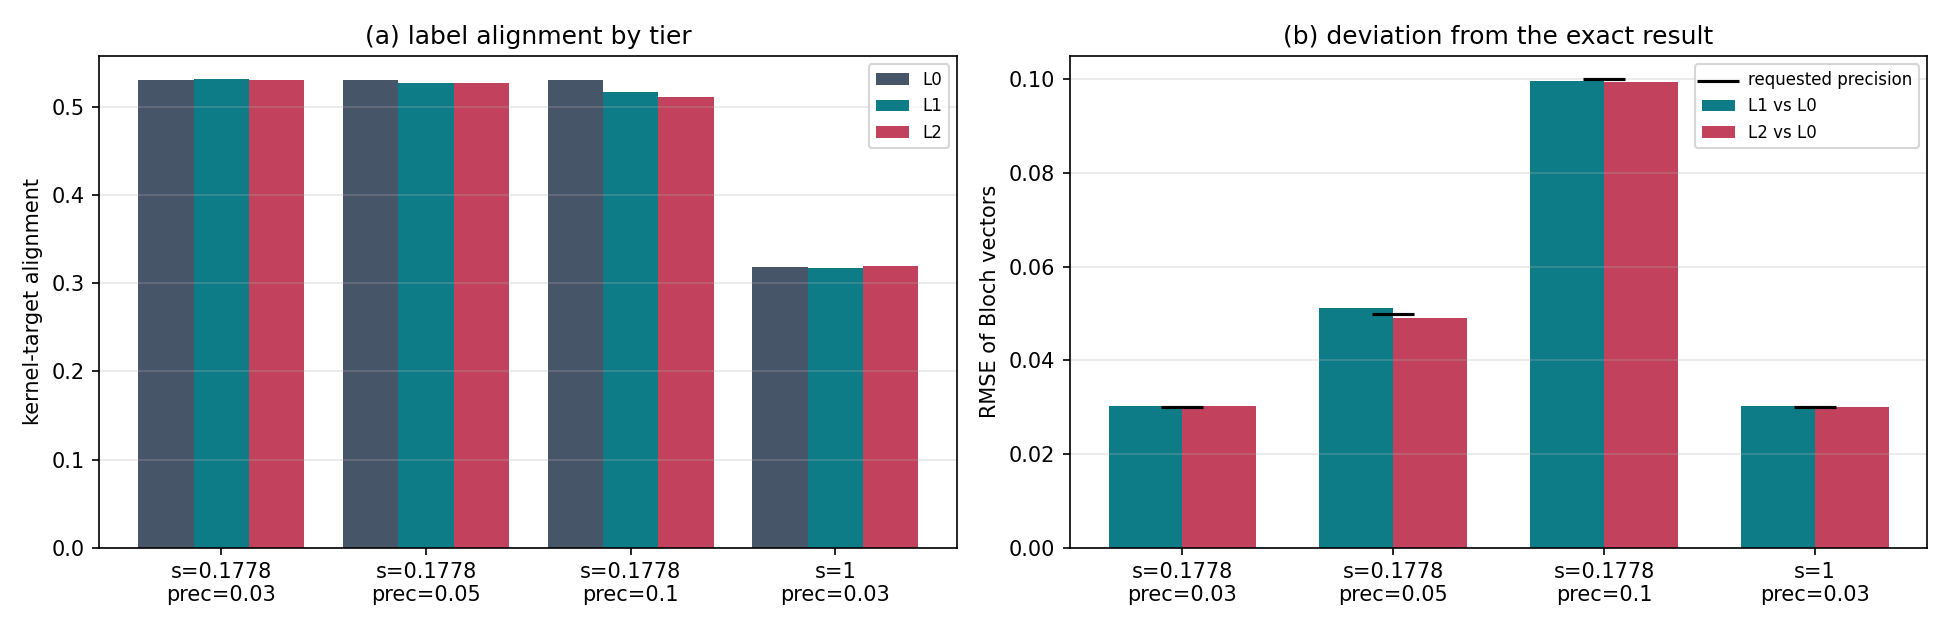
\includegraphics[width=0.8\textwidth]{fig/q06.png}
\caption{Q-06. (a) KTA per livello e configurazione. (b) Errore dei vettori di Bloch rispetto all’esatto; il trattino
nero è la precisione richiesta.}
\end{figure}

\textbf{Come leggere.} In (a), per $s=0{,}1778$ e precisione 0,03 le tre barre sono uguali (0,531 / 0,532 / 0,530): il
rumore non toglie informazione. A precisione 0,1 il calo diventa visibile (0,512 in L2); con $s=1$ tutto parte già
basso (0,32). In (b) l’errore coincide sempre con la precisione chiesta, anche con il rumore del chip.

\dire{“Glitch diversi producono vettori di Bloch che differiscono in media di 0,23, otto volte il rumore di misura:
per questo il rumore non cancella l’informazione. Era una previsione: la campagna l’ha confermata.”}

\attenzione{L2 non include la mitigazione di IBM, quindi è una previsione pessimistica.}

\subsection{Risultato 3 --- pilota su hardware (H-01)}
\textbf{Come.} 10 punti sintetici, 8 qubit, 2 strati, $s=1$, precisione 0,03, su \texttt{ibm\_kingston} con
mitigazione; gli stessi punti in L0, L1, L2. Corsa \texttt{hw-20261124T005515Z}.

\begin{figure}[H]
\centering
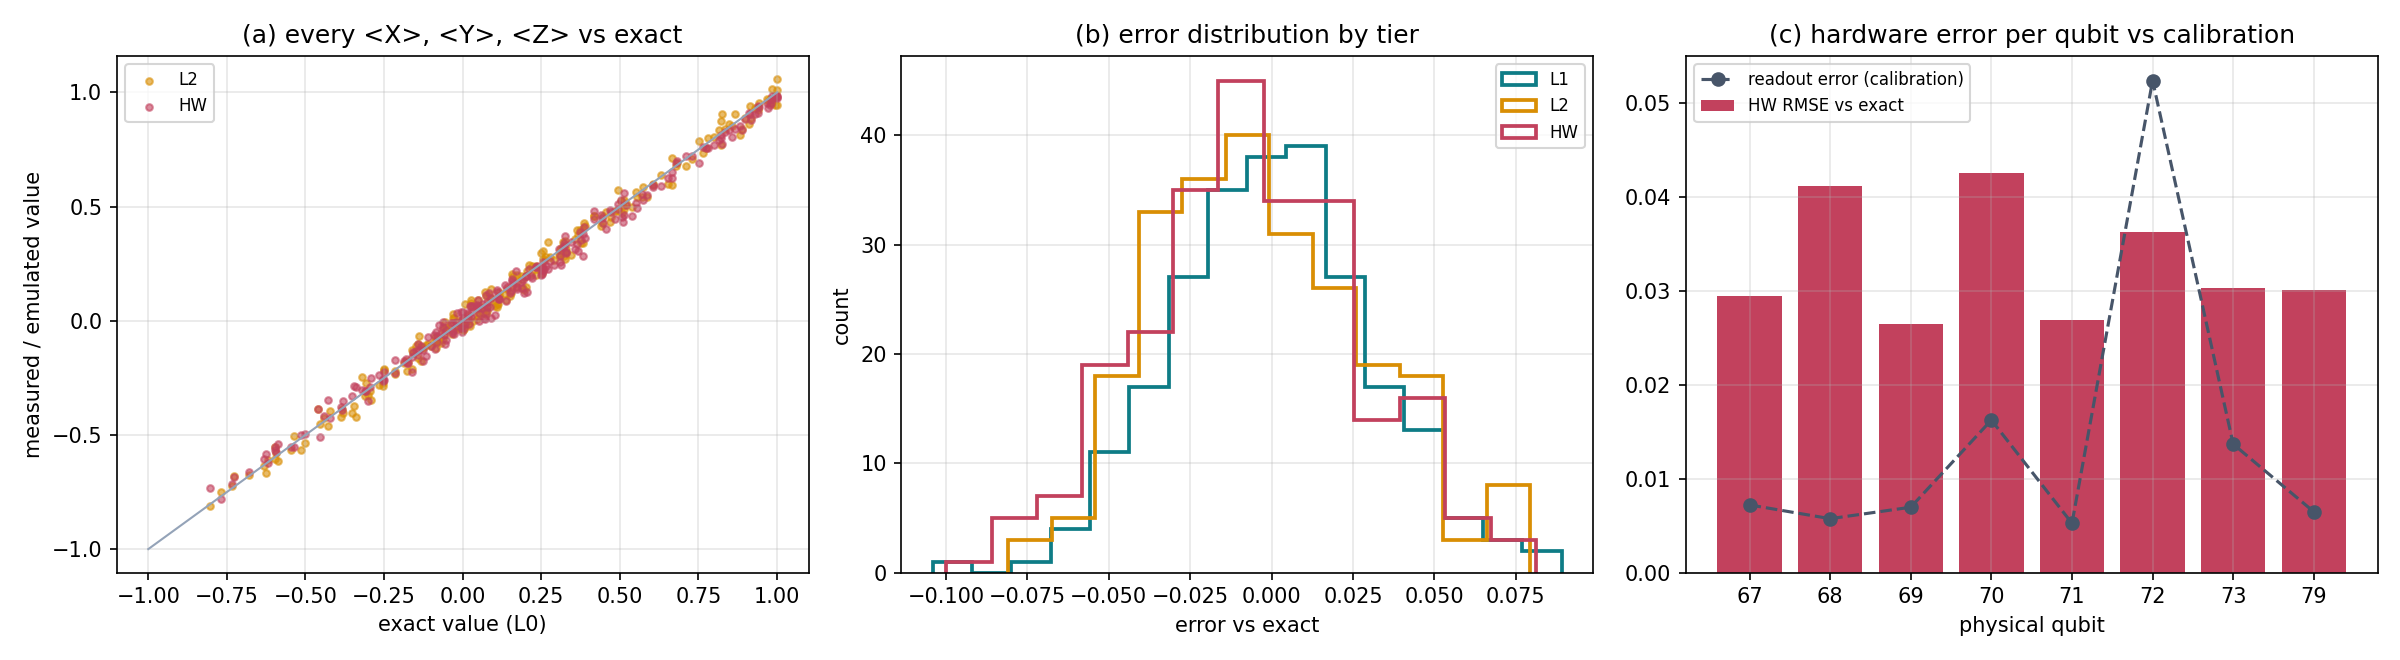
\includegraphics[width=\textwidth]{fig/h01.png}
\caption{H-01. (a) Valori misurati contro esatti. (b) Distribuzione degli errori per livello. (c) Errore per qubit
fisico confrontato con l’errore di lettura dichiarato da IBM.}
\end{figure}

\textbf{Come leggere.} (a) I 240 valori (10 punti $\times$ 8 qubit $\times$ 3 assi) stanno tutti sulla diagonale.
(b) Le curve dei tre livelli quasi coincidono, larghe circa $\pm0{,}05$. (c) Il qubit con l’errore di lettura peggiore
(5,2\%) non è il più impreciso: la correzione TREX funziona.

\dire{“13 secondi di QPU contro 13,7 previsti dalla formula IBM: possiamo pianificare il budget. L’errore
dell’hardware è 0,033 contro 0,030 del solo campionamento.”}

\attenzione{punti sintetici e un solo job: verifica la macchina, non la classificazione.}

\subsection{Risultato 4 --- la campagna hardware (H-02)}
\textbf{Come.} Configurazione congelata, sette esperimenti sui sottoinsiemi di D-05 (tabella~\ref{tab:campagna}),
corsa \texttt{hw-20261125T124523Z}. Una prima sottomissione (\texttt{hw-20261125T113624Z}) si è interrotta dopo
\emph{main}: la usiamo come ripetizione indipendente. Analisi: \texttt{experiments/h02\_analysis.py}, che legge solo lo
store.

\begin{table}[H]
\centering\small
\begin{tabular}{@{}lrrrl@{}}
\toprule
Esperimento & Glitch & Qubit & QPU (s) & Per misurare\\
\midrule
drift-start & 5 & 8 & 8 & riferimento di inizio\\
main (mitigato) & 120 & 8 & 124 & kernel e informazione sul chip\\
control (senza mitigazione) & 40 & 8 & 37 & effetto della mitigazione\\
concentration n4, n8, n12 & 3 $\times$ 30 & 4, 8, 12 & 3 $\times$ 33 & concentrazione sul chip\\
drift-end & 5 & 8 & 8 & deriva tra inizio e fine\\
\midrule
totale & 260 & & 276 & stimati 413 con margine\\
\bottomrule
\end{tabular}
\caption{La campagna H-02. 780 circuiti, 1112 shot ciascuno.}
\label{tab:campagna}
\end{table}

\begin{figure}[H]
\centering
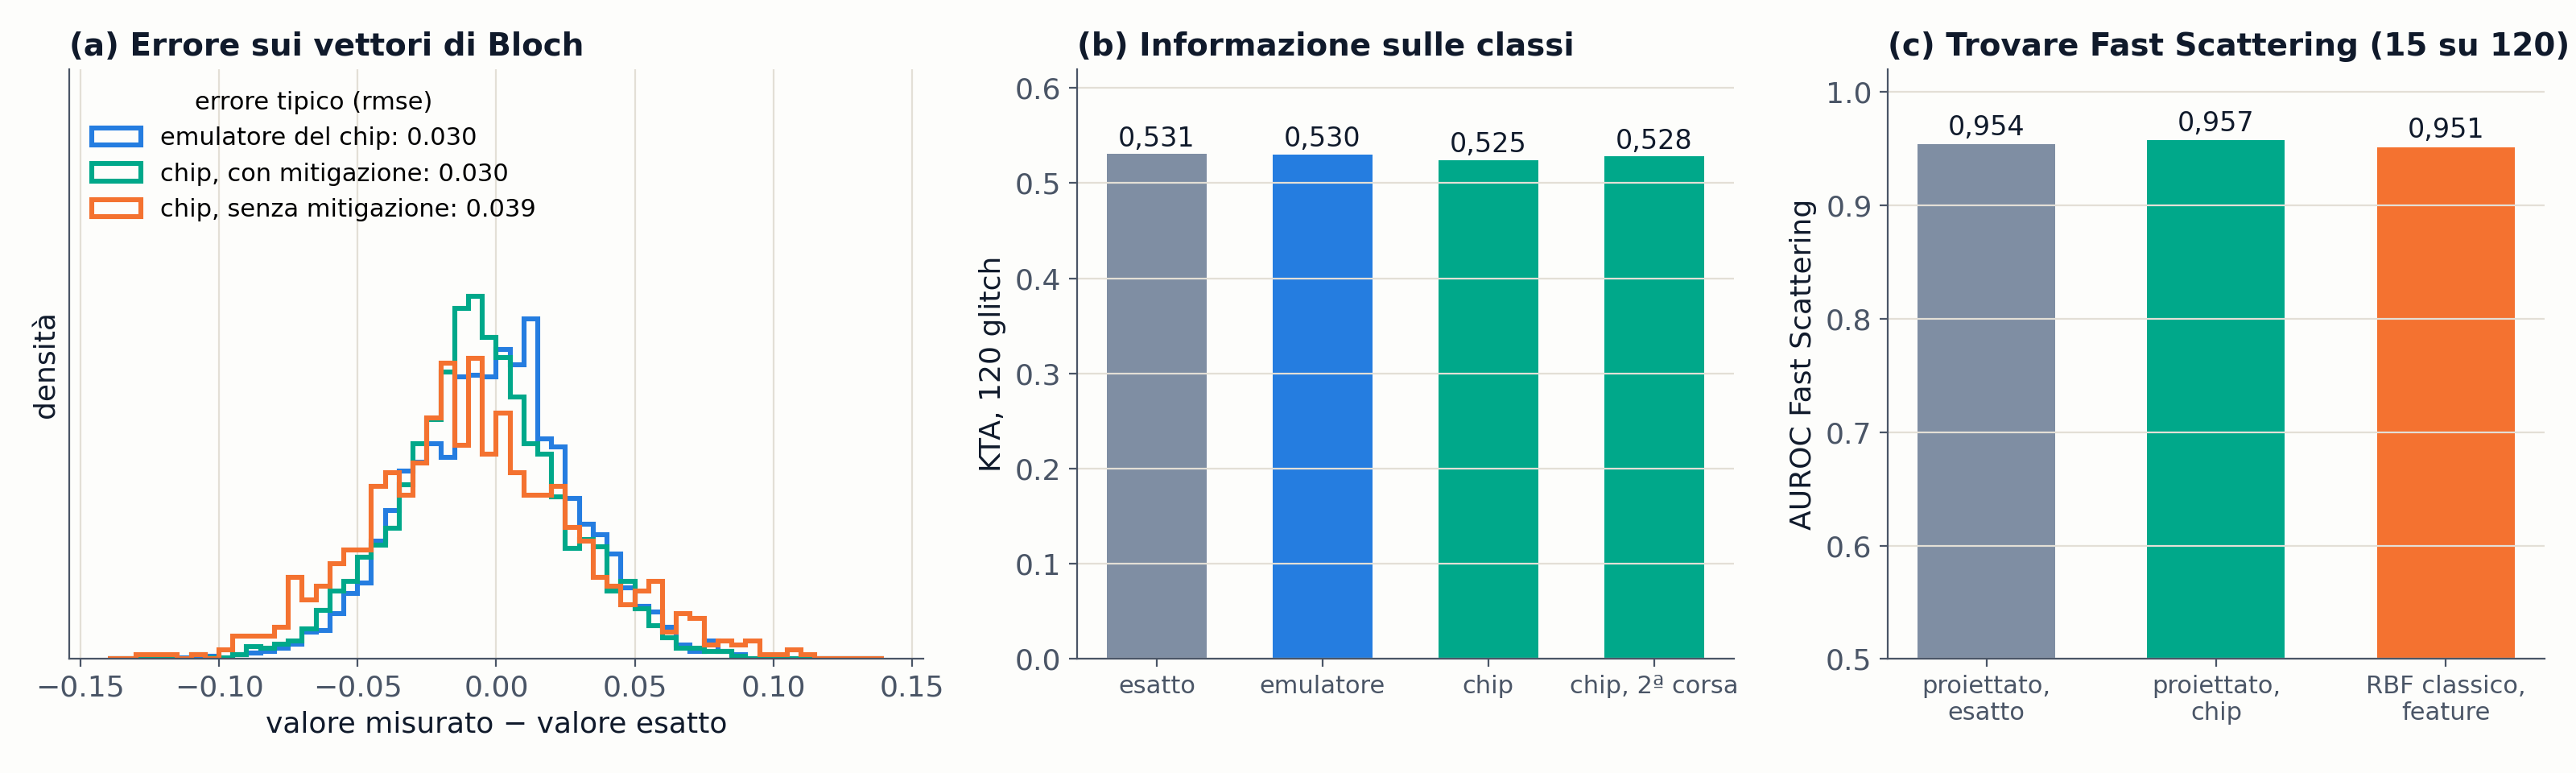
\includegraphics[width=\textwidth]{fig/h02_slide.png}
\caption{H-02. (a) Distribuzione dell’errore (misurato meno esatto) sulle componenti dei vettori di Bloch.
(b) KTA sui 120 glitch main. (c) AUROC per separare i 15 Fast Scattering dai 105 glitch noti.}
\label{fig:h02}
\end{figure}

\textbf{Come leggere (a).} Ogni curva è un istogramma di 2880 errori (120 glitch $\times$ 8 qubit $\times$ 3 assi). Blu:
emulatore; verde: chip con mitigazione; arancio: chip senza mitigazione (gruppo di controllo, 40 glitch, quindi meno
conteggi). Il numero in legenda è l’errore tipico (radice dell’errore quadratico medio). Con mitigazione il chip ha
0,030, uguale all’emulatore e al solo campionamento; senza sale a 0,039 e la curva è più larga e spostata a sinistra.

\textbf{Come leggere (b).} L’informazione sulle famiglie: 0,531 esatto, 0,530 emulatore, 0,525 chip, 0,528 seconda
corsa. Il chip perde circa l’1\%. È il test H4: differenza $-0{,}006$, intervallo bootstrap $[-0{,}010;\,-0{,}001]$,
tutto dentro la soglia di 0,02 fissata prima.

\textbf{Come leggere (c).} Anteprima di E-04: un One-Class SVM allenato su 2048 glitch noti (vettori esatti) dà un
punteggio ai 120 glitch main. Con i vettori misurati sul chip separa i 15 Fast Scattering con AUROC 0,957, come con
quelli esatti (0,954) e come un RBF classico sulle feature (0,951).

\dire{“Il chip vero si comporta come avevamo previsto: errore pari al campionamento, informazione intatta, e la
famiglia nuova si trova anche con i dati misurati.”}

\attenzione{nel pannello (c) i positivi sono solo 15: l’AUROC ha un’incertezza di qualche centesimo, e le tre barre sono
statisticamente indistinguibili. Il detector usa la scelta di $\gamma$ più frequente di E-03 ($c=31{,}6$) e $\nu=0{,}05$
senza ritaratura: è un’anteprima, non E-04.}

\begin{figure}[H]
\centering
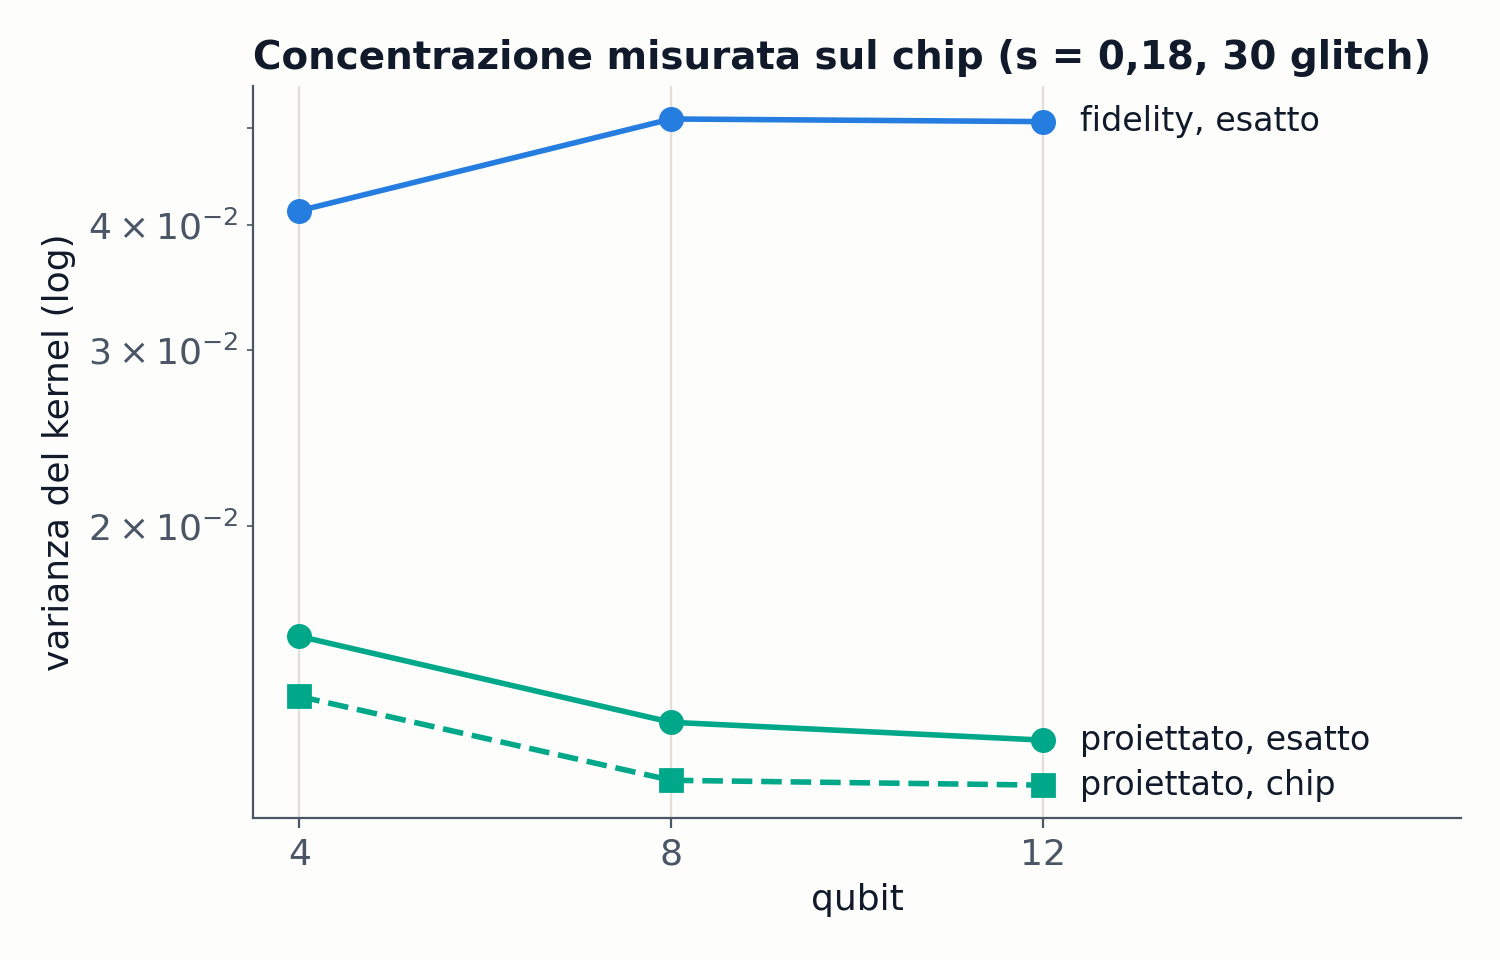
\includegraphics[width=0.62\textwidth]{fig/h02_conc.png}
\caption{Concentrazione misurata sul chip: varianza del kernel su 30 glitch, a 4, 8 e 12 qubit.}
\label{fig:h02conc}
\end{figure}

\textbf{Come leggere la figura~\ref{fig:h02conc}.} Verde pieno: proiettato in simulazione; verde tratteggiato:
proiettato sul chip, circa il 12\% più basso ma con lo stesso andamento; blu: fidelity in simulazione. Alla bandwidth
scelta nessuno dei due si concentra tra 4 e 12 qubit: il crollo di E-01 avveniva a $s=1$. Il rumore “accorcia” i
vettori di Bloch e quindi riduce un po’ le distanze, ma non appiattisce il kernel.

\textbf{Gli altri controlli.} Inizio contro fine campagna: differenza 0,034. Due corse diverse dello stesso main:
0,039. Entrambi sotto 0,042, che è quanto ci si aspetta dal solo campionamento confrontando due misure indipendenti
($\sqrt2\times0{,}03$): il chip non deriva in modo misurabile nei circa 10 minuti della campagna. Senza mitigazione il
chip aggiunge un errore suo di $\sqrt{0{,}039^2-0{,}030^2}\approx0{,}024$.

\subsection{Risultato 5 --- few-shot (anteprima di E-02)}
\textbf{Come.} Split P1 congelati, $k=5,10,20,50$ glitch per famiglia nota, 5 seed, 700 glitch di test (100 per
famiglia), simulazione esatta. SVM sul kernel proiettato contro SVM RBF sulle feature, 16 configurazioni di
iperparametri ciascuna. Script: \texttt{experiments/e2e\_l0.py --sweep} (L-04).

\begin{figure}[H]
\centering
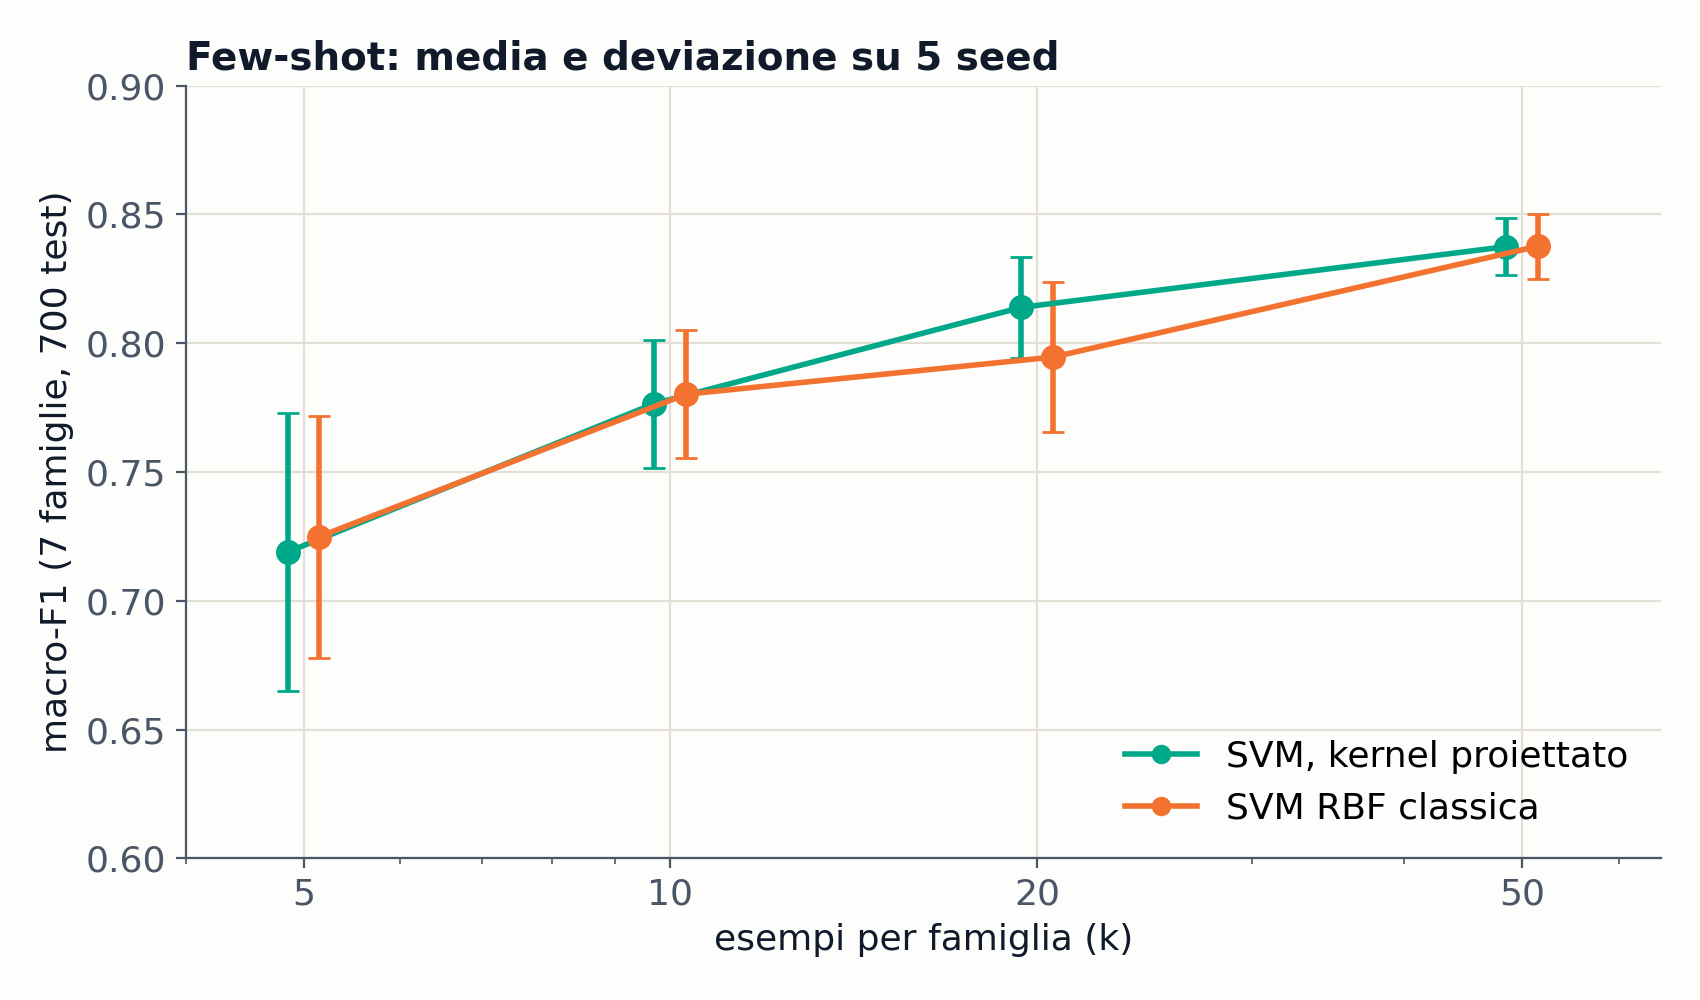
\includegraphics[width=0.62\textwidth]{fig/fewshot.png}
\caption{Few-shot: macro-F1 media e deviazione standard su 5 seed.}
\end{figure}

\textbf{Come leggere.} In ascissa gli esempi per famiglia (scala logaritmica), in ordinata la macro-F1. Le due curve
crescono insieme da circa 0,72 a 0,84 e le barre d’errore si sovrappongono a ogni $k$. Differenze medie: $-0{,}006$,
$-0{,}004$, $+0{,}019$, $0{,}000$.

\dire{“Con pochi esempi il kernel quantistico è alla pari con quello classico. È quello che chiedeva H1: non peggiore.”}

\attenzione{5 seed e un solo avversario: è un’anteprima. Il test pre-registrato usa 20 seed, il Wilcoxon appaiato e
tutte le baseline (k-NN, boosting, logistica, laplaciano).}

\subsection{Risultato 6 --- trovare la famiglia nuova (E-03)}
\textbf{Come.} Split P2: ogni famiglia a turno è “sconosciuta” e resta fuori da training, validazione, scaler e scelta
dei parametri; 10 seed, quindi 80 casi; al massimo 2048 glitch di training, 2048 di validazione, 8192 di test per caso.
I parametri si scelgono usando a turno ogni famiglia nota come anomalia di prova (leave-one-family-out annidato, con
lo scaler rifatto in ogni rotazione); $\gamma=c/\text{mediana delle distanze}$ con 9 valori di $c$; la soglia dà il 5\%
di falsi allarmi sulle sole famiglie note.

\begin{figure}[H]
\centering
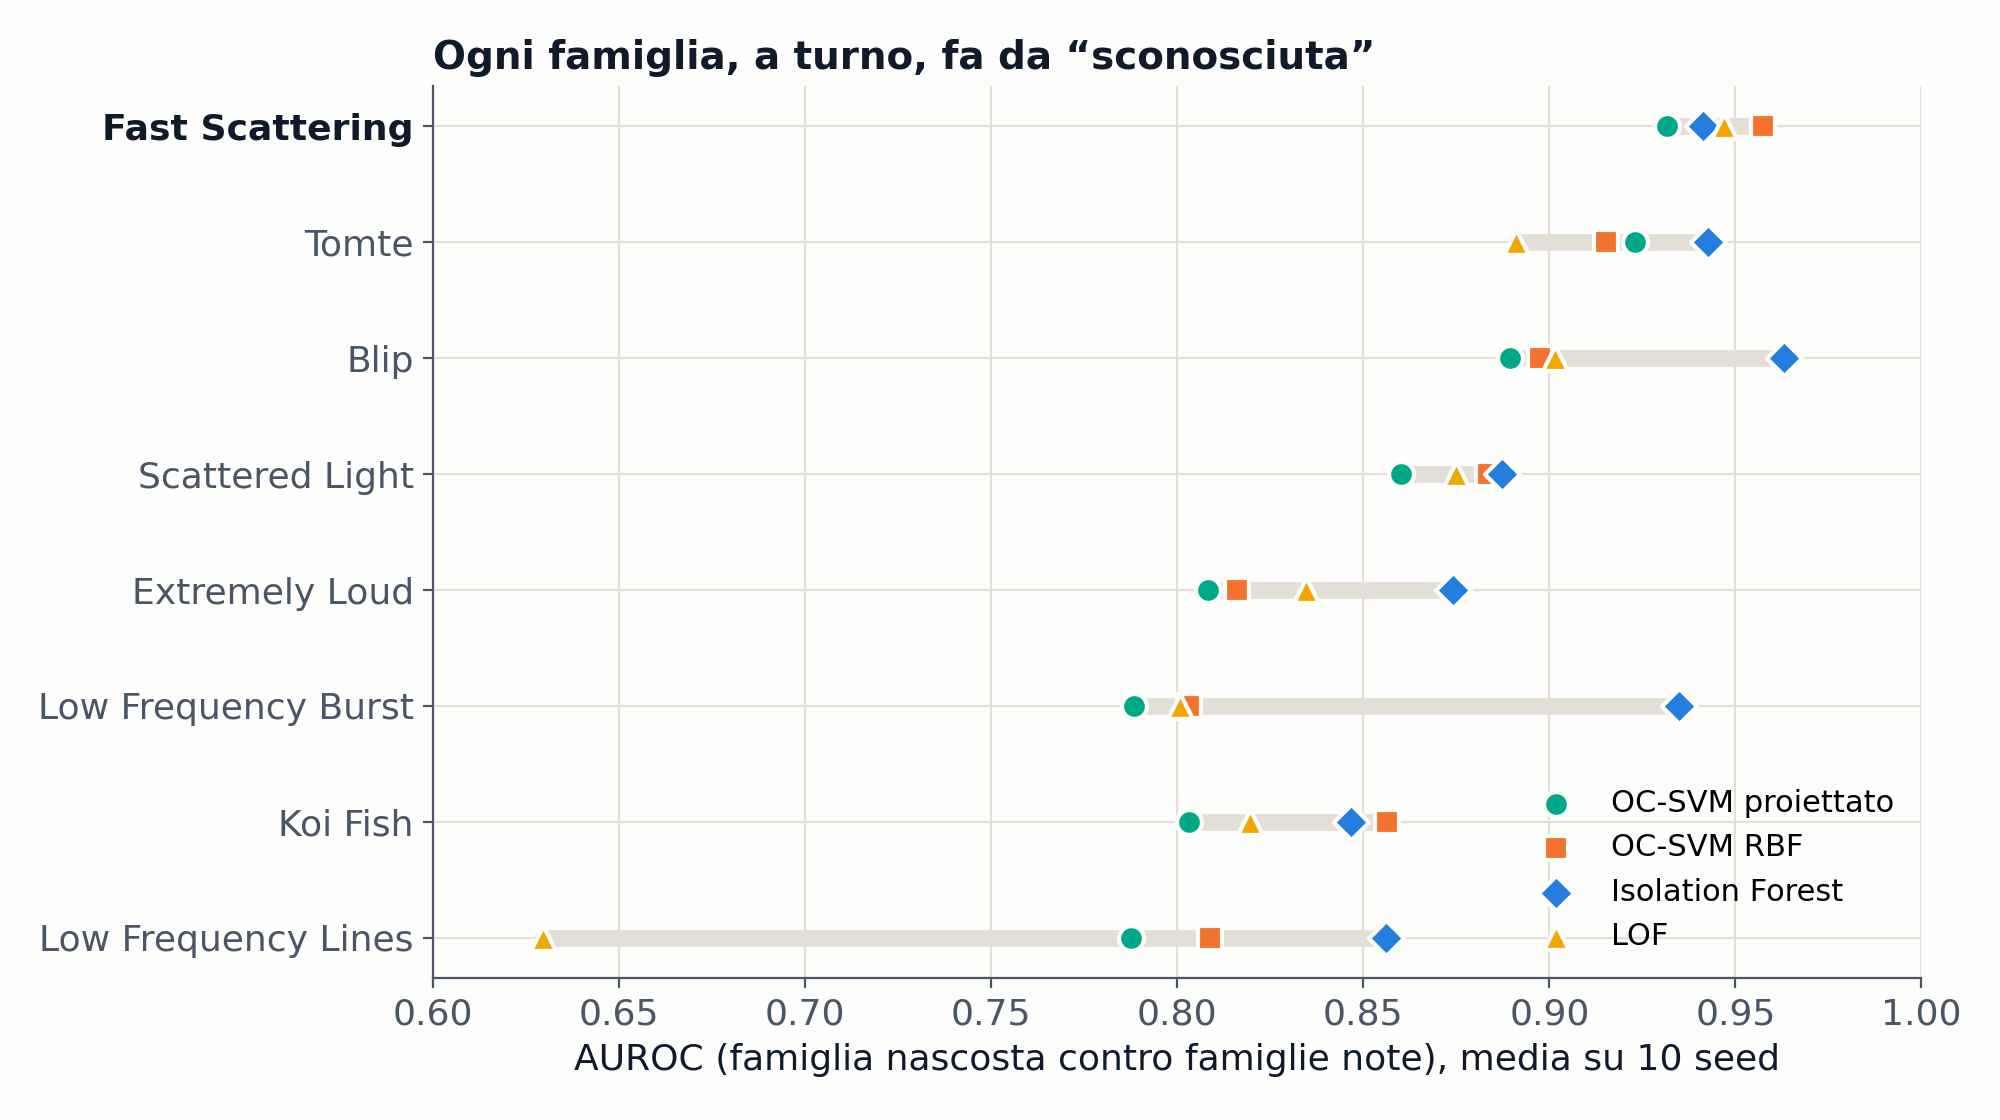
\includegraphics[width=0.75\textwidth]{fig/e03_families.png}
\caption{E-03. Per ogni famiglia tenuta nascosta, l’AUROC medio su 10 seed dei quattro detector.}
\end{figure}

\textbf{Come leggere.} Ogni riga è una famiglia nascosta; i simboli sono i quattro detector; la barra grigia va dal
peggiore al migliore. Più a destra è meglio. Per Fast Scattering tutti superano 0,93: proiettato 0,932, RBF 0,957,
Isolation Forest 0,941, LOF 0,947. La più difficile da riconoscere come nuova è Low Frequency Lines (media 0,77), seguita da
Koi Fish, Low Frequency Burst ed Extremely Loud (circa 0,83). Nessuno degli 80 casi ha AUROC sotto 0,5.

\dire{“Tutti i detector riconoscono Fast Scattering come nuova. Ma il confronto appaiato è chiaro: l’RBF classico fa
meglio del proiettato di 0,026, e l’intervallo non contiene lo zero. H3 non è supportata.”}

\attenzione{E-03 è in simulazione esatta. I risultati sono condizionati al test fissato e alle cap di 2048/8192 glitch.
Le famiglie note sono state usate a turno come anomalie, ma condividono dati: le 8 rotazioni non sono 8 esperimenti
indipendenti. Il budget di ricerca è un tetto di 60 (OC-SVM 54, Isolation Forest 60, LOF 15): il confronto principale,
proiettato contro RBF, è comunque 54 contro 54. Questa deviazione va approvata e scritta in \texttt{decisions.md}.}

\subsection{I risultati hanno senso?}
Ogni riga è una previsione scritta prima e confrontata dopo:
\begin{center}
\begin{tabular}{@{}lrr@{}}
\toprule
Controllo & Previsto & Misurato\\
\midrule
costo QPU della campagna & 318\,s (formula IBM, senza margine) & 276\,s\\
errore dei vettori, con mitigazione & 0,030 (L2) & 0,030\\
KTA sui 120 glitch & 0,530 (L2) & 0,525\\
due corse indipendenti & $\leq0{,}042$ & 0,039\\
deriva in circa 10 minuti & $\leq0{,}042$ & 0,034\\
AUROC Fast Scattering, esatto e chip & uguali & 0,954 e 0,957\\
\bottomrule
\end{tabular}
\end{center}
E un controllo che ha trovato un nostro errore: la prima versione di E-03 sceglieva $\gamma$ guardando solo il tasso di
falsi allarmi; il risultato erano AUROC sotto 0,5 in 55 casi su 320 (peggio del caso). Abbiamo cambiato il criterio
(AUROC su famiglie note usate come anomalie) prima di guardare l’hardware, e lo dichiariamo come rianalisi.

\section{Verdetto, possibili vantaggi, futuro}

\textbf{Verdetto.} Due risultati positivi: la parte quantistica funziona sull’hardware con costo e rumore previsti, e
il kernel proiettato evita la concentrazione. Un risultato negativo: su questi dati nessun vantaggio sul classico.
È coerente con Bowles et al.\ (2024): con 7 feature e 8 qubit tutto è simulabile su un laptop, e un RBF ben tarato è
un avversario fortissimo.

\textbf{Dove potrebbe esserci un vantaggio.} (i) Input più ricchi: spettrogrammi e canali ausiliari invece di 7 numeri.
(ii) Scale non simulabili: molti più qubit e circuiti più profondi, dove però il rumore cresce. (iii) Uno screening
preventivo: la geometric difference dice prima di spendere QPU se un kernel quantistico può battere il classico.

\textbf{Lavoro futuro.} E-04 completo (novelty sui vettori del chip, con più Fast Scattering e $\gamma$ ritarato);
few-shot completo (H1 e H2 con 20 seed); 14--16 qubit con studio del rumore; feature più ricche; geometric difference
su ogni dataset; detector alternativi sullo stesso kernel (densità, k-NN, kernel PCA, issue \#69).

\section{Come abbiamo costruito il progetto}
Cinque persone: un lead e quattro aree (dati, quantum e hardware, machine learning, diagnostica ed esperimenti). Ogni
task una issue, ogni modifica una pull request revisionata (circa 70). Prima i contratti d’interfaccia
(\texttt{docs/contracts.md}) e dei dati sintetici, così tutti potevano lavorare in parallelo dal primo giorno. Circa 290
test automatici. Ogni risultato è salvato con hash dei dati, commit del codice e configurazione: si rigenera con un
comando. Struttura: \texttt{data/} $\to$ \texttt{features/} $\to$ \texttt{quantum/} $\to$ \texttt{store/} $\to$
\texttt{kernels/} $\to$ \texttt{models/}, con \texttt{diagnostics/} ed \texttt{experiments/} sopra.


\section{Discussione e limiti}
\textbf{Positivo.} La pipeline porta dati astrofisici reali su un chip IBM con costo e rumore previsti in anticipo;
il kernel proiettato evita la concentrazione nel regime studiato; il rumore hardware mitigato non riduce in modo
rilevante l’informazione sulle classi (H4) né la capacità di trovare Fast Scattering (anteprima E-04).

\textbf{Negativo.} Nessun vantaggio sul classico: pari nel few-shot (anteprima, H1), peggiore nella novelty (H3).
Coerente con Bowles et al.\ (2024) e con l’osservazione di Cerezo et al.\ (2023): a 8 qubit e con 7 feature il modello
è simulabile e un RBF ben tarato è un avversario fortissimo.

\textbf{Limiti.} Etichette ML di Gravity Spy, non verità fisica; Fast Scattering confusa con il rivelatore L1 e con O3;
E-03 con cap di 2048/2048/8192 glitch per caso e intervalli condizionati al test; budget di ricerca della novelty come
tetto (54/60/15), da approvare come deviazione; anteprime few-shot (5 seed) ed E-04 (15 positivi, $\gamma$ non
ritarato); correzione di Holm su H1--H4 non ancora applicata; H2 non testata; un solo chip in un solo giorno.

\appendix
\section{Ogni numero e da dove viene}
\label{app:numeri}

\begin{center}\small
\begin{tabularx}{\textwidth}{@{}>{\raggedright\arraybackslash}X r >{\raggedright\arraybackslash}p{6.2cm}@{}}
\toprule
Numero & Valore & Fonte (script e run)\\
\midrule
glitch curati, 8 famiglie & 318.801 & \texttt{data/curate.py}, D-02\\
Fast Scattering (di cui su L1) & 56.509 (55.229) & \texttt{docs/E03\_results.md}\\
KTA proiettato, $s=0{,}1778$ / $s=1$ & 0,534 / 0,357 & \texttt{results/e01/e01\_gravityspy.csv}\\
KTA fidelity, $n=8$ & 0,557 & idem\\
KTA L0/L1/L2 sui 120 main & 0,531 / 0,532 / 0,530 & \texttt{results/q06/q06\_main.csv}\\
pilota: QPU misurati / formula & 13\,s / 13,7\,s & \texttt{hw-20261124T005515Z}, \texttt{docs/qpu\_policy.md}\\
pilota: errore HW / L1 & 0,033 / 0,030 & idem\\
campagna: QPU misurati / stima & 276\,s / 413\,s & \texttt{hw-20261125T124523Z}, \texttt{results/campaign/}\\
errore main con / senza mitigazione & 0,030 / 0,039 & \texttt{results/h02/h02\_experiments.csv}\\
KTA main esatto / L2 / HW / ripetizione & 0,531 / 0,530 / 0,525 / 0,528 & \texttt{results/h02/}, ripetizione \texttt{hw-20261125T113624Z}\\
H4: $\Delta$KTA [IC 95\%] & $-0{,}006$ $[-0{,}010;\,-0{,}001]$ & \texttt{results/h02/h02\_summary.json}\\
deriva / ripetizione & 0,034 / 0,039 & idem\\
AUROC FS sui 120: esatto / HW / RBF & 0,954 / 0,957 / 0,951 & idem (anteprima E-04)\\
few-shot macro-F1, $k=50$, proiettato / RBF & 0,838 / 0,838 & \texttt{results/e2e/fewshot\_sweep.csv} (L-04)\\
E-03 AUROC FS: proiettato / RBF / IF / LOF & 0,932 / 0,957 / 0,941 / 0,947 & branch E-03, \texttt{results/e03/e03\_metrics.csv}\\
E-03 differenza appaiata [IC 95\%] & $-0{,}026$ $[-0{,}044;\,-0{,}008]$ & branch E-03, \texttt{e03\_paired\_differences.csv}\\
\bottomrule
\end{tabularx}
\end{center}

\textbf{Configurazione congelata} (\texttt{configs/hardware\_frozen.yaml}, tag \texttt{hw-freeze}): 8 qubit, 2 strati,
$s=0{,}1778$, precisione 0,03 (1112 shot), \texttt{ibm\_kingston}, scaler P2 seed 0, concentrazione a 4/8/12 qubit.


\section{Riferimenti}
\begin{itemize}
  \item S. Bahaadini et al., \emph{Machine learning for Gravity Spy: glitch classification and dataset}, Information
  Sciences 444 (2018).
  \item J. Bowles, S. Ahmed, M. Schuld, \emph{Better than classical? The subtle art of benchmarking quantum machine
  learning models}, arXiv:2403.07059 (2024).
  \item M. Cerezo et al., \emph{Does provable absence of barren plateaus imply classical simulability?},
  arXiv:2312.09121 (2023).
  \item J. Glanzer et al., \emph{Data quality up to the third observing run of Advanced LIGO: Gravity Spy glitch
  classifications}, Class.\ Quantum Grav.\ 40 (2023).
  \item V. Havlíček et al., \emph{Supervised learning with quantum-enhanced feature spaces}, Nature 567 (2019).
  \item H.-Y. Huang et al., \emph{Power of data in quantum machine learning}, Nature Communications 12 (2021).
  \item M. Schuld, N. Killoran, \emph{Quantum machine learning in feature Hilbert spaces}, Phys.\ Rev.\ Lett.\ 122 (2019).
  \item S. Soni et al., \emph{Discovering features in gravitational-wave data through detector characterization,
  citizen science and machine learning}, Class.\ Quantum Grav.\ 38 (2021).
  \item S. Thanasilp et al., \emph{Exponential concentration in quantum kernel methods}, Nature Communications 15 (2024).
  \item Y. Wu et al., \emph{Advancing glitch classification in Gravity Spy: multi-view fusion with attention-based machine
  learning for Advanced LIGO’s fourth observing run}, arXiv:2401.12913 (2024).
  \item M. Zevin et al., \emph{Gravity Spy: integrating Advanced LIGO detector characterization, machine learning, and
  citizen science}, Class.\ Quantum Grav.\ 34 (2017).
\end{itemize}


\end{document}
